\label{chap6}
To be able to evaluate the proposed solution in a real-life scenario, a prototype based on the concept presented was built. This chapter introduces the implementation from a high level
view, followed by the evaluation of the result. Afterwards, the results are discussed and improvements are suggested.
\subsection{Implementation}
The necessary software, running on each platform, is written in the programming language "C". To interface with \gls{knx}, an \gls{api} named "EIBD" is used, providing functions to
send \gls{knx} frames to and receive frames from the bus. "EIBD" offers synchronous as well as asynchronous calls for sending and receiving frames. While the first kind of
call will block until the operation finished, the second kind of call will return immediately, the status of such calls can be checked by another special "EIBD" call.
Because it is not possible to use callbacks with asynchronous calls, the implementation uses the synchronous functions. Because every platform possess 3 distinct interfaces to the bus (2 interfaces form the redundant "secure" part of the network, one is connected
to a standard \gls{knx} network), care must be taken that no frames are missed while the main logic is blocked. This can be achieved by splitting the main program into different 
processes or alternatively, threads, where for each critical task, a distinct part is responsible. While threads share the same address space and thus facilitating communication with
each other, processes rely on special functions to be able
to communicate with each other. Additionally, thread-creation and switching between threads consumes less computing resources. Therefore, it was decided to choose the multi-threaded
approach. Consequently, at least 3 different threads - one for each communication interface - are needed. Nevertheless, because every thread must be able to write to \textit{or} receive
frames from the bus at unpredictable moments, 7 different threads are used: the main thread only handles argument processing and creates the other threads. For the remaining threads,
two pairs are responsible for the interfaces to the secured network, while the remaining thread pair handles writing to and reading from the bus. This setup is shown in Figure 

\begin{figure}
\centering
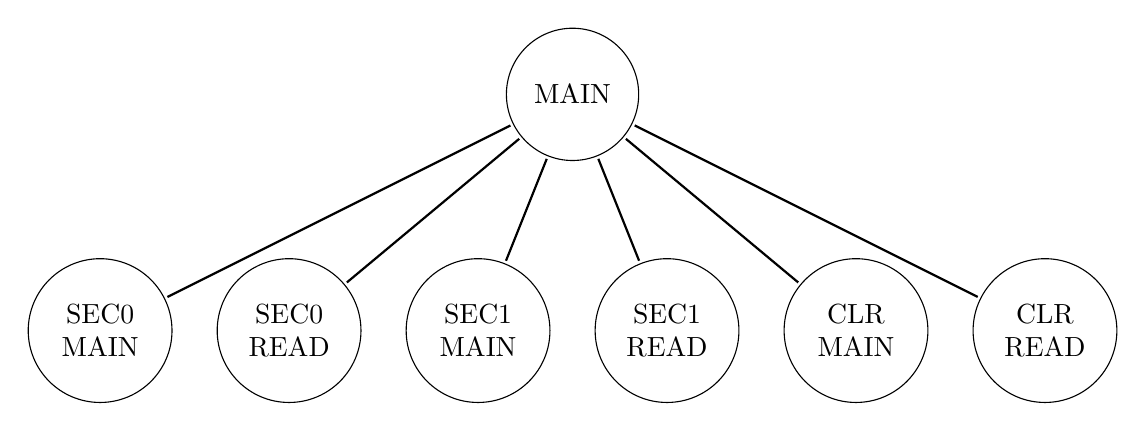
\begin{tikzpicture}[scale=0.2]
\tikzstyle{every node}+=[inner sep=2pt]
\tikzstyle{arrow}=[draw, -latex] 
\tikzset{
    pil/.style={
           ->,
           thick,
           shorten <=1pt,
           shorten >=1pt,}
}
\usetikzlibrary{automata,positioning}
\usetikzlibrary{positioning}
\node[state,text width=1.5cm,align=center]					at (-10,5)		(m)			{MAIN}; 
\node[state,text width=1.5cm,align=center]					at (-40,-10)	(sec0m)	{SEC0 MAIN}; 
\node[state,text width=1.5cm,align=center]					at (-28,-10)	(sec0r)		{SEC0 READ}; 
\node[state,text width=1.5cm,align=center]					at (-16,-10)	(sec1m)	{SEC1 MAIN}; 
\node[state,text width=1.5cm,align=center]					at (-4,-10)		(sec1r)		{SEC1 READ}; 
\node[state,text width=1.5cm,align=center]					at (8,-10)	(clrm)		{CLR MAIN}; 
\node[state,text width=1.5cm,align=center]					at (20,-10)	(clrr)			{CLR READ};
\path[pil,-] (m)  edge[auto]   node[] {} (sec0m); 
\path[pil,-] (m)  edge[auto]   node[] {} (sec0r); 
\path[pil,-] (m)  edge[auto]   node[] {} (sec1m); 
\path[pil,-] (m)  edge[auto]   node[] {} (sec1r); 
\path[pil,-] (m)  edge[auto]   node[] {} (clrm); 
\path[pil,-] (m)  edge[auto]   node[] {} (clrr); 

%\path[pil,->] (sec0r)  edge[auto, out=240, in=300]   node[] {} (sec0m); 
%\path[pil,->] (sec1r)  edge[auto, out=240, in=300]   node[] {} (sec1m); 
%\path[pil,->] (clrr)  edge[auto, out=210, in=290]   node[] {} (sec1m); 
%\path[pil,->] (clrr)  edge[auto, out=230, in= 180]   node[] {} (sec0m); 
\end{tikzpicture}
\label{fig:threads}
\caption{Threads used in the implementation}
\end{figure}


\subsubsection{KNX addressing scheme}

Care must be taken that no duplicate \gls{knx} addresses are used within the network. Therefore, the following addressing convention is proposed:
While it would be possible to use the same addresses on both lines per gateway, a different scheme is used.
For the secured network, the address ranges starting at address 1.1.1 to address 1.1.15 and 1.2.1 to 1.2.15 are reserved for secure line number
1 and 2 respectively, which allows a maximum of 15 gateways. Different addresses are used mainly because it facilitates debugging. 
On the unsecured lines, every gateway uses an address from the range 1.0.1 - 1.0.15. Addresses are assigned in a linearly ascending way, so gateway number 1
uses addresses 1.1.1 and 1.2.1 for secure lines 1 and 2, and 1.0.1 for its unsecured line.

\subsection{\gls{mac2} generation}

The \gls{ttl} field cannot be included in the \gls{mac2} calculation because this field gets changed by a router and would therefor invalidate an authentic message.

\subsection{EIBD \gls{api}}

Use VBusMonitor to receive packets, this way EIBD can L2 acknowledge individual-, group- and broadcast frames
\\
\\
For sending individual packages, use EIBOpenT\_Individual(con, myAddr, FALSE)
\\
\\
For sending group packages, use EIBOpen\_GroupSocket(con, TRUE) and EIBSendGroup(con, dest, size, buf)
\\
\\
For sending broadcast packages, use EIBOpenT\_Broadcast(con, TRUE) and EIBSendAPDU(con, size, buf)

\subsection{Restrictions }

EIBD can send extended frames, but can not receive frames with payload >= 56 byte. 

\subsection{FIXMEs}

\begin{enumerate}
 \item DH: apply hashingfunction on derived secret to get 2 different keys(MAC, encrypt)
 \item 
\end{enumerate}



\section{Evaluation}

\subsection{\gls{usb}}
Unstable \gls{usb} connection, enumeration errors, to fix reboot hub

\subsection{Synchronization phase}
Packages in the synchronization phase are not encrypted, allowing a passive adversary to learn the value of the global counter value $Ctr_{global}$. Nevertheless,
this counter is only used to avoid deterministic encryption (see \ref{deterministicEnc}) and is of no use for the attacker.
\\
\\
Opening a window for tolerating timing deviations allows an active attacker to inject a captured synchronization response package within that time window.
Nevertheless, because the header is protected by a \gls{mac2}, the only way to inject a synchronization package is to use exactly the same frame as captured,
i.e. the same source address, which will be discarded because the the requesting device already finished the synchronization stage.
\\
Additionally, the counter value is of no use for the attacker, as described above.

\subsection{Discovery phase}

\subsection{Data transmission phase}


\subsection{High Level Cryptography Library}

\subsubsection{OpenSSL}

\begin{itemize}
 \item install libssl, libssl-dev
\end{itemize}

